\documentclass{article}
\usepackage[margin=1in, paperwidth=30cm, paperheight=20cm]{geometry}

\usepackage{xparse}
\usepackage{tikz}
\usepackage{ifthen}
\usetikzlibrary{calc,positioning}
\usetikzlibrary{automata,arrows} 
\usetikzlibrary{fit,chains}
%%%
%draw input/output boxes
%used by record
%
%example:
%	\def\mar{v1,v2}
%
%	\RecordBox{ \mar }{1}{rec}
%
\tikzset{input/.style={anchor=north west}}
\tikzset{output/.style={anchor=north east}}
\tikzset{rbox/.style={rectangle,draw}}

\def\getlen#1{%
\pgfmathsetmacro{\lenarray}{0}% 
\foreach \i in #1{%
\pgfmathtruncatemacro{\lenarray}{\lenarray+1}% 
\global\let\lenarray\lenarray}%
}   
\NewDocumentCommand{\RecordBox}{m m m}{%var list,1=input/2=output, rec
	\getlen{ #1 }
	\begin{scope}[start chain=going below,node distance=-0.02cm]
	\foreach \v [count=\i] in #1 {
		\ifthenelse{\i=1}{
			\ifthenelse{#2=1}{
	    		\path let 
					\p1=($(#3.west)-(#3.east)$),
				 	\p2=($(#3.north)-(#3.south)$),
            	  	\n1 = {veclen(\p1)*0.16} 					%width
			  		,\n2 = {veclen(\p2)/\lenarray} 					%height
              		in node[on chain, rbox, input
			  		  ,minimum width=\n1
					  ,minimum height=\n2
					  ] (#3\v) at (#3.north west) {\v};
			}{
	    		\path let 
					\p1=($(#3.west)-(#3.east)$),
				 	\p2=($(#3.north)-(#3.south)$),
            	  	\n1 = {veclen(\p1)*0.16} 					%width
			  		,\n2 = {veclen(\p2)/\lenarray} 					%height
              		in node[on chain, rbox, output
			  		  ,minimum width=\n1
					  ,minimum height=\n2
					  ] (#3\v) at (#3.north east) {\v};

			}
		}{
    		\path let 
				\p1=($(#3.west)-(#3.east)$),
			  	\p2=($(#3.north)-(#3.south)$),
              	\n1 = {veclen(\p1)*0.16} 					%width
			  	,\n2 = {veclen(\p2)/\lenarray} 					%height
              	in node[on chain, rbox
			  		  ,minimum width=\n1
					  ,minimum height=\n2
					  ,anchor=north
					  ] (#3\v) {\v};
		}
	}
	\end{scope}
}


\newcounter{image}
\setcounter{image}{0}
\pgfmathtruncatemacro{\recordwidth}{4}
\pgfmathtruncatemacro{\recordheight}{2}

\newcommand{\setrecordwidth}[1]{\pgfmathtruncatemacro{\recordwidth}{#1}}
\newcommand{\setrecordheight}[1]{\pgfmathtruncatemacro{\recordheight}{#1}}

\tikzset{drawinside/.code n args={3}{%
		%
		%% input box
		\RecordBox{ #2 }{1}{#1}
%
		%% output box
		\RecordBox{ #3 }{2}{#1}
    }
}

\tikzset{record/.style args={#1 and #2}{
        rectangle,draw,minimum width=#1, minimum height=#2
    }
}

\NewDocumentCommand{\drawrecord}{d() m m m m}{ %1. coord. [optional], recname, input var., output var., automat name
\stepcounter{image}
\IfNoValueTF{#1}{%true
\node[record=\recordwidth cm and \recordheight cm,name=a#2,
fit=(#5)]{};
}
{%false
\node[record=\recordwidth cm and \recordheight cm,name=a#2, inner
sep =\recordwidth * 0.15cm,
fit=(#5)] at (#1){};
}
\node[drawinside={a#2}{#3}{#4}] (A) at (a#2.center)
{};
}

\NewDocumentCommand{\connect}{m m}{
\draw[->] (#1) -- (#2);
}


\begin{document}
%\tikz{\drawrecord{v_1}{v_2}{o_1}}
%\tikz{\drawrecord{v_4}{v_5}{o_2}}

%\vspace*{2cm}
%
%to set:
%1: pos of records (here: a1(0,0) and a2(10,0)
%2: create automata as node like 'autom'
%3: set input and output variables
%
\begin{tikzpicture}
\node (autom) at (0,0) { 			%automata 1 as tikzpicture
	\begin{tikzpicture}[>=stealth',shorten >=1pt,auto,node distance=3 cm,
		scale = 1, transform shape]
		\node[initial,state] (A) {};

		\path[->] (A) edge [loop below] node [align=center]  {$c=c+1$} (A)
	    		  (A) edge [loop above]node [align=center]  {$c=c+5$} (A);
	\end{tikzpicture}
};
\node (autom1) at (10,0) { 			%automata 2 as tikzpicture
	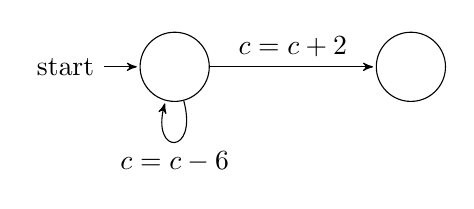
\begin{tikzpicture}[>=stealth',shorten >=1pt,auto,node distance=3 cm,
		scale = 1, transform shape]
		\node[initial,state] (A) {};
		\node[state] (B) at ++(3,0) {};

		\path[->] (A) edge [loop below] node [align=center]  {$c=c-6$} (A)
				  (A) edge node [align=center] {$c=c+2$} (B);
	\end{tikzpicture}
};

\drawrecord(0,0){ {i1,i2} }{ {o1} }{autom} 	%create record a1 
\drawrecord(10,0){ {a,b} }{ {o} }{autom1} 	%create record a2
\connect{a1o1}{a2a} 					%access I/O variables by using its recordname + variablenames
\end{tikzpicture}
\end{document}
